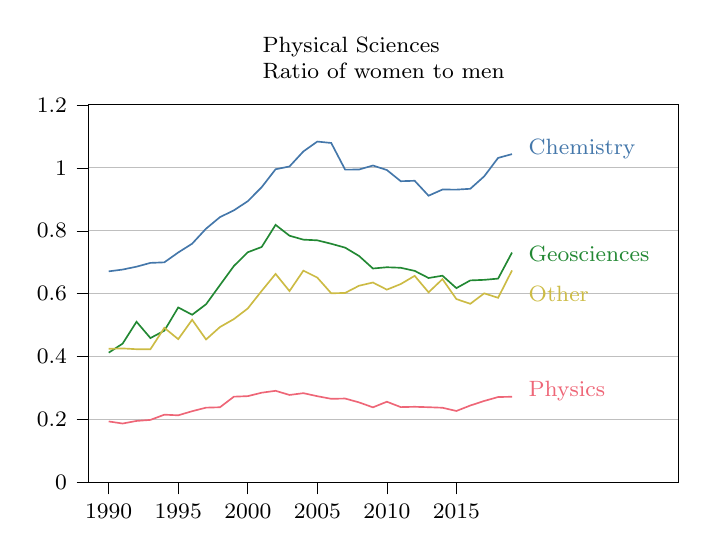
\begin{tikzpicture}[every node/.style={font=\footnotesize},
align=left]
% This file was created with tikzplotlib v0.9.17.
\definecolor{color0}{rgb}{0.266666666666667,0.466666666666667,0.666666666666667}
\definecolor{color1}{rgb}{0.933333333333333,0.4,0.466666666666667}
\definecolor{color2}{rgb}{0.133333333333333,0.533333333333333,0.2}
\definecolor{color3}{rgb}{0.8,0.733333333333333,0.266666666666667}

\begin{axis}[
height=6.376357092455836cm,
tick align=outside,
tick pos=left,
title={Physical Sciences \\ Ratio of women to men},
width=9.079103cm,
x grid style={white!69.0196078431373!black},
xmin=1988.55, xmax=2031,
xtick style={color=black},
xtick={1990,1995,2000,2005,2010,2015},
xticklabels={
  \(\displaystyle 1990\),
  \(\displaystyle 1995\),
  \(\displaystyle 2000\),
  \(\displaystyle 2005\),
  \(\displaystyle 2010\),
  \(\displaystyle 2015\)
},
ymajorgrids,
ymin=0, ymax=1.2,
ytick style={color=black},
ytick={0,0.2,0.4,0.6,0.8,1,1.2},
yticklabels={
  \(\displaystyle 0\),
  \(\displaystyle 0.2\),
  \(\displaystyle 0.4\),
  \(\displaystyle 0.6\),
  \(\displaystyle 0.8\),
  \(\displaystyle 1\),
  \(\displaystyle 1.2\)
}
]
\addplot [semithick, color0]
table {%
1990 0.671039354187689
1991 0.676785714285714
1992 0.685910915694896
1993 0.69794776119403
1994 0.699717713479181
1995 0.731048805815161
1996 0.75900641552887
1997 0.806735235567352
1998 0.843441226575809
1999 0.864903759669005
2000 0.894080996884735
2001 0.938588279348437
2002 0.995605273671594
2003 1.00445253997167
2004 1.05229565575458
2005 1.08357799960853
2006 1.07913799348062
2007 0.994340878828229
2008 0.994725063938619
2009 1.00745688985552
2010 0.993175614194722
2011 0.957595659623073
2012 0.958948215723102
2013 0.911496467565832
2014 0.931158969251836
2015 0.93084181773032
2016 0.933491390067382
2017 0.973075510953372
2018 1.03163331181407
2019 1.04367449887163
};
\addplot [semithick, color1]
table {%
1990 0.194038406420178
1991 0.187412587412587
1992 0.195633187772926
1993 0.198942109903027
1994 0.215477996965099
1995 0.213540018981335
1996 0.22656508777741
1997 0.237869390733309
1998 0.239068100358423
1999 0.272727272727273
2000 0.274450341167551
2001 0.285370879120879
2002 0.291399229781772
2003 0.278211284513806
2004 0.283905458638154
2005 0.274263904034896
2006 0.265949462096572
2007 0.266808712121212
2008 0.254617722702829
2009 0.238819732595666
2010 0.256713700500683
2011 0.23959673959674
2012 0.240569823434992
2013 0.239245835621453
2014 0.237533039647577
2015 0.227295534370296
2016 0.244655200128597
2017 0.259088010204082
2018 0.271610624904038
2019 0.272494733674391
};
\addplot [semithick, color2]
table {%
1990 0.412641621943948
1991 0.441265976871576
1992 0.510834236186349
1993 0.45903165735568
1994 0.482448630136986
1995 0.556327160493827
1996 0.533155487804878
1997 0.56638198757764
1998 0.627360469995804
1999 0.68796992481203
2000 0.7317429406037
2001 0.748560460652591
2002 0.818825910931174
2003 0.784333672431333
2004 0.771822358346095
2005 0.769706336939722
2006 0.758743030917385
2007 0.746450304259635
2008 0.720018665422305
2009 0.680118946474087
2010 0.684106222750694
2011 0.682439537329127
2012 0.672641509433962
2013 0.649957032368949
2014 0.657241931181648
2015 0.617704280155642
2016 0.642288196958726
2017 0.644059644059644
2018 0.648034107058266
2019 0.730911005792522
};
\addplot [semithick, color3]
table {%
1990 0.42483660130719
1991 0.426124197002141
1992 0.423603793466807
1993 0.423517169614984
1994 0.491578947368421
1995 0.455522971652004
1996 0.517167381974249
1997 0.454545454545455
1998 0.494079655543595
1999 0.519343493552169
2000 0.553086419753086
2001 0.608958837772397
2002 0.662933930571109
2003 0.608324439701174
2004 0.673349056603774
2005 0.651209677419355
2006 0.601332064700285
2007 0.602455146364495
2008 0.625346901017576
2009 0.635593220338983
2010 0.612959719789842
2011 0.630742049469965
2012 0.656804733727811
2013 0.604386677497969
2014 0.646360759493671
2015 0.582999198075381
2016 0.567901234567901
2017 0.601132686084142
2018 0.587025316455696
2019 0.673986486486487
};
\draw (axis cs:2019.5,1.04367449887163) node[
  anchor=base west,
  text=color0,
  rotate=0.0
]{Chemistry};
\draw (axis cs:2019.5,0.272494733674391) node[
  anchor=base west,
  text=color1,
  rotate=0.0
]{Physics};
\draw (axis cs:2019.5,0.700911005792522) node[
  anchor=base west,
  text=color2,
  rotate=0.0
]{Geosciences};
\draw (axis cs:2019.5,0.573986486486487) node[
  anchor=base west,
  text=color3,
  rotate=0.0
]{Other};
\end{axis}



\end{tikzpicture}

\caption{Source: IPEDS.}
